\title{Relazione di ``Metodi del Calcolo Scientifico''}
\author{
	Simon Vocella \\
	Matricola: 718289
}
\date{\today}

% TODO [LD] teoria
% OK [LD] jtransform
% OK [LD] i listati dei programmi
% OK [LD] risultati
% OK [LD] conclusioni

% TODO [DCT2] teoria
% OK [DCT2] jtransform
% OK [DCT2] i listati dei programmi
% OK [DCT2] risultati
% OK [DCT2] conclusioni

\documentclass[12pt]{article}
\usepackage[margin=1.5cm]{geometry}
\usepackage[italian]{babel}
\usepackage{booktabs}
\usepackage{algorithm}% http://ctan.org/pkg/algorithm
\usepackage{algpseudocode}% http://ctan.org/pkg/algorithmicx
\usepackage{algorithmicx}
\usepackage{lipsum}% http://ctan.org/pkg/lipsum
\usepackage{float}% http://ctan.org/pkg/float
\usepackage{graphicx}
\usepackage{amsfonts}
\usepackage{amsmath}
\usepackage{graphicx}

\usepackage{listings}
\lstset{language=Java, basicstyle=\small}
\lstset{linewidth=\textwidth, showstringspaces=false}
\lstset{frame=trBL}

\begin{document}
\maketitle

\section{Lu Decomposition}

\subsection{Teoria}

\subsection{Jama}
JAMA \`e un pacchetto di algebra lineare di base per Java. Fornisce le classi a livello di utente per la costruzione e la manipolazione di matrici reali, dense. \`E pensato per fornire funzionalit\`a sufficienti per problemi di routine, confezionati in un modo tale che sia naturale e comprensibile anche ai non esperti. \\
\\
Sono disponibili cinque scomposizioni fondamentali della matrice JAMA:
\begin{itemize}
\item La decomposizione di Cholesky, matrici simmetriche definite positive
\item Decomposizione LU (eliminazione gaussiana) di matrici rettangolari (Quella che usiamo in questo caso)
\item Decomposizione QR di matrici rettangolari
\item Decomposizione autovalore di matrici quadrate e simmetriche sia nonsymmetric
\item Valore Singolare decomposizione di matrici rettangolari
\end{itemize}
Funzionalit\`a non coperte: JAMA non \`e affatto un ambiente completo algebra lineare. Per esempio, non supporta matrici con struttura particolare o per ulteriori decomposizioni specializzati (ad esempio Shur, autovalore generalizzato). Matrici complesse non sono incluse. \\

\subsection{Programma lu-decomposition}
Per il progetto ho deciso di utilizzare Jama, perch\`e sembra essere veloce e semplice da implementare, alla fine non mi ha deluso, tranne forse il fatto che non supporta i valori complessi e non ho potuto calcolare gli autovalori delle matrici rand, che ho lasciato ad n.a.\\
Qui \`e listato il programma principale.

\newpage
\lstinputlisting[caption=lu-decompostion,label=lst:java]{../../lu-decomposition/src/Main.java}

\newpage

\subsection{Risultati e conclusioni}
Qui presentiamo i valori dei test precedenti con cui dovremmo confrontare i valori ottenuti.\\
Come vediamo quando viene calcolato l'errore relativo e l'errore sulla prima componente, manteniamo lo stesso ordine di grandezza nella maggior parte di casi, perdiamo o guadagniamo un ordine di grandezza nel caso di matrici bad e very bad. \\
Nel caso del calcolo del settimo autovalore i risultati sono praticamente gli stessi. \\
Nei valori ottenuti abbiamo aggiunto due colonne: Time to solve che \`e il tempo di calcolo della lu-decomposition e il tempo di calcolo degli autovalori. \\
Come vediamo entrambi i tempi si matengono bassi tranne nel caso di rand-5000 per il tempo di calcolo della lu-decomposition e eig-5000 nel caso del calcolo degli autovalori. \\

\begin{table}[h]
\caption {Valori dei test precedenti} \label{tab:title}
\begin{center}
\begin{tabular}{|l|r|r|r|}
\hline
Test         &	Errore Relativo  &	Errore Prima Comp  & Autovalore n.7 \\
\hline
     easy-10 &	    4.242156e-016 &	     6.661338e-016 &  				 7.000000 \\
    easy-100 &	    2.019904e-015 &	     3.330669e-015 &           7.000000 \\
   easy-1000 &	    2.654198e-014 &	     1.554312e-014 &           7.000000 \\
     rand-10 &	    5.607561e-015  &	   1.132427e-014 &               n.a. \\
    rand-100 &	    8.760746e-014 &	     2.065015e-014 &               n.a. \\
   rand-1000 &	     3.827585e-012 &	   5.317968e-013 &               n.a. \\
   rand-5000 &	   1.102259e-011   &	   1.227463e-012 &               n.a. \\
      bad-10 &	    6.287577e-007  &	   4.387160e-007 &           5.999999 \\
     bad-100 &	    9.304715e-006 &	     9.864899e-006 &           6.000000 \\
     bad-500 &	    8.763526e-005 &	     8.822490e-005 &           5.999999 \\
    bad-1000 &	    7.556303e-005 &	     7.484208e-005 &           5.999999 \\
  verybad-10 &	    5.264102e-005 &	     4.405734e-005 &           6.000000 \\
 verybad-100 &	    1.197916e-003 &	     1.140304e-003 &           6.000000 \\
 verybad-500 &	    2.451563e-003 &	     2.454550e-003 &           6.000000  \\
verybad-1000 &	    1.921933e-002 &	     1.907311e-002 &           6.000000 \\
      eig-10 &	            n.a. &	              n.a. &           1.212788 \\
      eig-20 &	            n.a. &	              n.a. &           0.616452  \\
      eig-30 &	            n.a. &	              n.a. &           0.386165 \\
      eig-40 &	            n.a. &	              n.a. &           0.251158  \\
      eig-50 &	            n.a. &	              n.a. &           0.183589  \\
     eig-100 &	            n.a. &	              n.a. &           0.105820 \\
    eig-1000 &	            n.a. &	              n.a. &           0.005791 \\
    eig-2000 &	            n.a. &	              n.a. &           0.004094 \\
    eig-5000 &	            n.a. &	              n.a. &           0.001635 \\
\hline
\end{tabular}
\end{center}
\end{table}
\begin{table}[h]
\caption {Valori Ottenuti} \label{tab:title}
\begin{center}
\begin{tabular}{|l|r|r|r|r|r|}
\hline
Test         &	Errore Relativo  &	Errore Prima Comp  & Autovalore n.7    &	Time to solve &	Time to calc. eigen \\
\hline
     easy-10 &	    3.510833e-16 &	      2.220446e-16 &           7.000000 & 	0ms		 	 &		0ms   \\
    easy-100 &	    2.853360e-15 &	      1.110223e-15 &           7.000000 & 	1ms		 	 &		0ms   \\
   easy-1000 &	    3.174443e-14 &	      3.264056e-14 &           7.000000 &	670ms		 &		9ms   \\
     rand-10 &	    4.711062e-15 &	      8.659740e-15 &               n.a. & 	0ms		 	 &		0ms   \\
    rand-100 &	    1.001901e-13 &	      8.237855e-14 &               n.a. & 	1ms		 	 &		0ms   \\
   rand-1000 &	    2.547025e-12 &	      4.767298e-13 &               n.a. &	647ms		 &		0ms   \\
   rand-5000 &	    9.787832e-12 &	      1.521339e-11 &               n.a. &	101418ms	 &		0ms   \\
      bad-10 &	    3.118816e-07 &	      2.176155e-07 &           6.000000 & 	0ms		 	 &		0ms   \\
     bad-100 &	    2.258293e-05 &	      2.394252e-05 &           6.000000 & 	1ms		 	 &		0ms   \\
     bad-500 &	    4.622912e-05 &	      4.654016e-05 &           6.000000 &	69ms		 &		2ms   \\
    bad-1000 &	    2.279306e-04 &	      2.257559e-04 &           6.000000 &	645ms		&		13ms   \\
  verybad-10 &	    4.993346e-04 &	      4.179128e-04 &           6.000000 & 	0ms		 	&		0ms   \\
 verybad-100 &	    3.283544e-03 &	      3.125627e-03 &           6.000000 & 	2ms		 	&		0ms   \\
 verybad-500 &	    1.065932e-02 &	      1.067230e-02 &           6.000000 &	70ms		 &		1ms   \\
verybad-1000 &	    2.926093e-02 &	      2.903832e-02 &           6.000000 &	644ms		 &		8ms   \\
      eig-10 &	            n.a. &	              n.a. &           1.212788 & 	0ms		 	&		0ms   \\
      eig-20 &	            n.a. &	              n.a. &           0.616452 & 	0ms		 &			0ms   \\
      eig-30 &	            n.a. &	              n.a. &           0.386165 & 	0ms		 &			0ms   \\
      eig-40 &	            n.a. &	              n.a. &           0.251158 & 	0ms		 &			0ms   \\
      eig-50 &	            n.a. &	              n.a. &           0.183589 & 	0ms		 &			0ms   \\
     eig-100 &	            n.a. &	              n.a. &           0.105820 & 	0ms		 &			1ms   \\
    eig-1000 &	            n.a. &	              n.a. &           0.005791 & 	0ms		 &			7ms   \\
    eig-2000 &	            n.a. &	              n.a. &           0.004094 & 	0ms		&			30ms   \\
    eig-5000 &	            n.a. &	              n.a. &           0.001635 &	0ms		&			967ms   \\
\hline
\end{tabular}
\end{center}
\end{table}

\newpage

\section{Discrete Cosine Transform}
\subsection{Teoria}
\subsection{JTransforms}
JTransforms \`e la prima, open source, multithreaded libreria FFT scritta in puro Java. Attualmente, quattro tipi di trasformazioni sono disponibili: Discrete Fourier Transform (DFT), Discrete Cosine Transform (DCT), Discrete Sine Transform (DST) e Discrete Hartley Transform (DHT).\\
\\
Caratteristiche:
\begin{itemize}
\item L'implementazione pi\`u veloce di DFT, DCT, DST e DHT in puro Java.
\item trasformazioni a 1, 2 e 3 dimensioni
\item Dimensione arbitraria dei dati.
\item Singola e doppia precisione.
\item Varianti Uni-dimensionale e multi-dimensionale di trasformazioni 2D e 3D.
\item Multithreading automatico - i thread sono utilizzati automaticamente se il numero di CPU > 1.
\item FFT ottimizzate per i dati di input reali (40\% pi\`u veloce che con i dati complessi).
\end{itemize}
Limitazioni:
\begin{itemize}
\item Il numero di thread deve essere una potenza di due.
\item Sono disponibili solo in-place trasformazioni.
\item Solo DCT-II-III e DCT sono disponibili.
\item Solo DST-II-III e DST sono disponibili.
\item Solo DHT reale \`e disponibile.
\end{itemize}

\subsection{Programma discrete-cosine-transform}
Per il progetto ho deciso di utilizzare JTransforms come implementazione FAST.\\
Qui \`e listato della classe che gestisce la mia implementazione di dct sia unidemensionale che bidimensionale.

\lstinputlisting[caption=discrete-cosine-transform,label=lst:java]{../src/Dct.java}

\subsection{Risultati e conclusioni}
Nella tabella riportata qui sotto ho messo i risultati dei benchmark sia della mia implementazione che di Jtransforms.
Notiamo la grande differenza nei tempi di computazione sia dovuta al fatto che Jtransforms utilizza multithread sia anche per l'implementazione FAST.
\\\\
\begin{figure}[htbp]
\centering
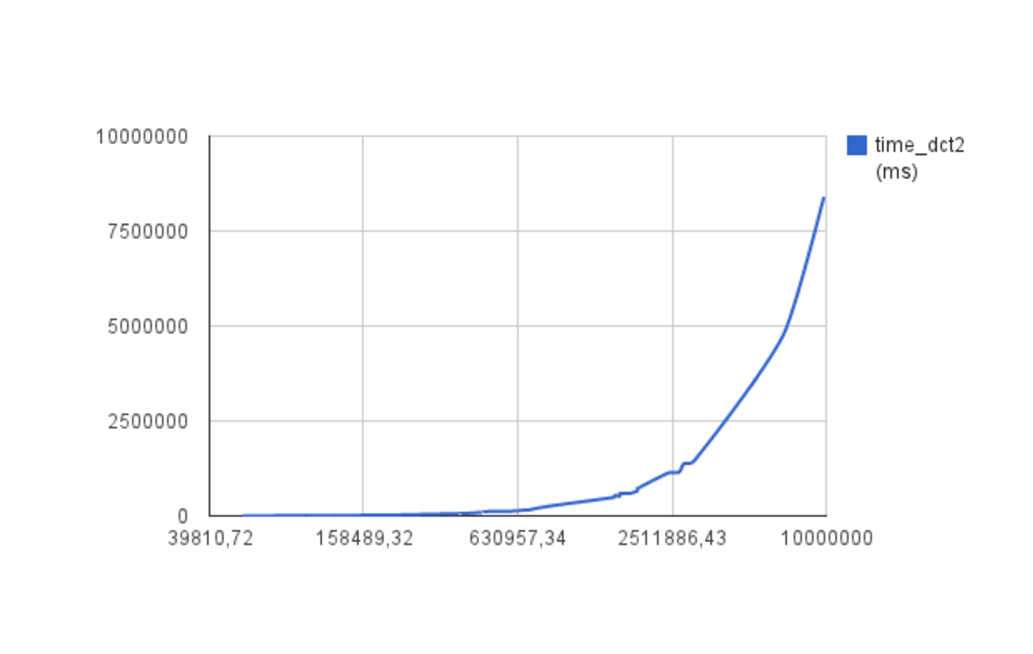
\includegraphics{grafico_dct2.eps}
\caption{Grafico dct2 implementata}
\end{figure}
\\\\
\begin{figure}[htbp]
\centering
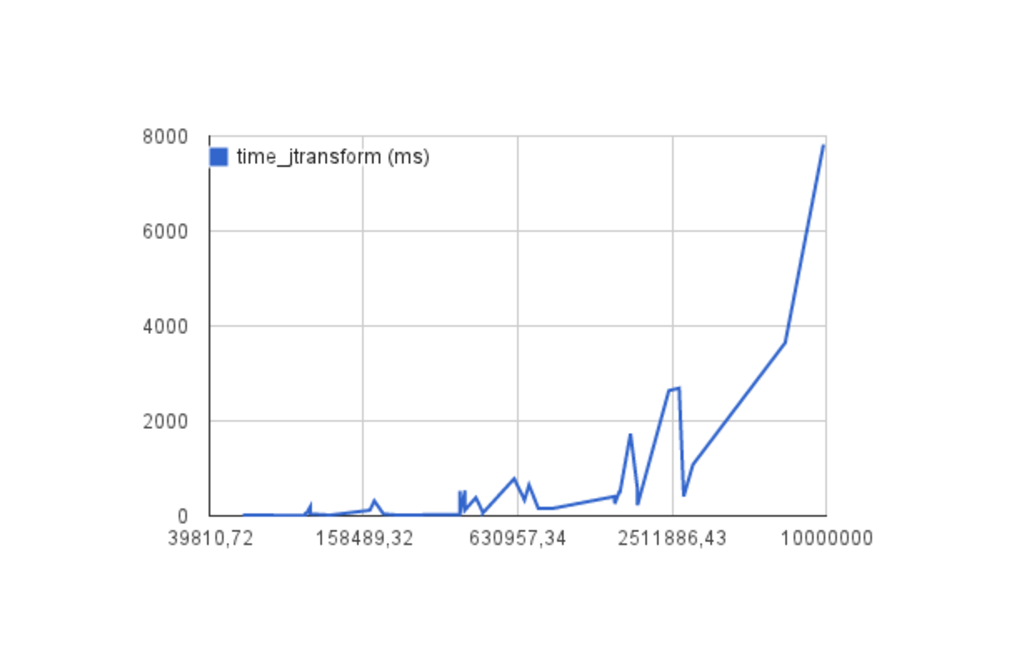
\includegraphics{grafico_jtransform.eps}
\caption{Grafico dct2 FAST}
\end{figure}
\\\\
\begin{table}[!h]
\begin{tabular}{|l|r|r|r|r|}
\hline
Name & Time Dct2 (ms) & Time Jt. (ms) & width (px) & height (px) \\ 
\hline
scaled/scaled/scaled/artificial.bmp & 7942 & 193 & 384 & 256 \\ 
scaled/scaled/scaled/big\_building.bmp & 127478 & 783 & 902 & 677 \\ 
scaled/scaled/scaled/big\_tree.bmp & 81907 & 383 & 761 & 569 \\ 
scaled/scaled/scaled/bridge.bmp & 19125 & 316 & 344 & 507 \\ 
scaled/scaled/scaled/cathedral.bmp & 7479 & 79 & 250 & 376 \\ 
scaled/scaled/scaled/deer.bmp & 18021 & 118 & 506 & 331 \\ 
scaled/scaled/scaled/fireworks.bmp & 10058 & 19 & 392 & 294 \\ 
scaled/scaled/scaled/flower\_foveon.bmp & 3284 & 18 & 284 & 189 \\ 
scaled/scaled/scaled/hdr.bmp & 7875 & 40 & 384 & 256 \\ 
scaled/scaled/scaled/leaves\_iso\_200.bmp & 7438 & 10 & 376 & 250 \\ 
scaled/scaled/scaled/leaves\_iso\_1600.bmp & 7551 & 10 & 376 & 250 \\ 
scaled/scaled/scaled/nightshot\_iso\_100.bmp & 10080 & 33 & 392 & 294 \\ 
scaled/scaled/scaled/nightshot\_iso\_1600.bmp & 10245 & 10 & 392 & 294 \\ 
scaled/scaled/scaled/spider\_web.bmp & 22486 & 38 & 532 & 356 \\ 
scaled/scaled/scaled/zone\_plate.bmp & 7588 & 8 & 375 & 250 \\ 
scaled/scaled/artificial.bmp & 66245 & 534 & 768 & 512 \\ 
scaled/scaled/big\_building.bmp & 1135163 & 2639 & 1804 & 1354 \\ 
scaled/scaled/big\_tree.bmp & 597656 & 1731 & 1522 & 1138 \\ 
scaled/scaled/bridge.bmp & 157433 & 650 & 688 & 1014 \\ 
scaled/scaled/cathedral.bmp & 60869 & 118 & 500 & 752 \\ 
scaled/scaled/deer.bmp & 151674 & 335 & 1012 & 662 \\ 
scaled/scaled/fireworks.bmp & 82743 & 82 & 784 & 588 \\ 
scaled/scaled/flower\_foveon.bmp & 25788 & 17 & 568 & 378 \\ 
scaled/scaled/hdr.bmp & 63813 & 125 & 768 & 512 \\ 
scaled/scaled/leaves\_iso\_200.bmp & 60658 & 527 & 752 & 500 \\ 
scaled/scaled/leaves\_iso\_1600.bmp & 61871 & 68 & 752 & 500 \\ 
scaled/scaled/nightshot\_iso\_100.bmp & 82330 & 111 & 784 & 588 \\ 
scaled/scaled/nightshot\_iso\_1600.bmp & 111011 & 59 & 784 & 588 \\ 
scaled/scaled/spider\_web.bmp & 207638 & 161 & 1064 & 712 \\ 
scaled/scaled/zone\_plate.bmp & 60285 & 29 & 750 & 500 \\ 
scaled/artificial.bmp & 518198 & 535 & 1536 & 1024 \\ 
scaled/big\_building.bmp & 8364020 & 7823 & 3608 & 2708 \\ 
scaled/big\_tree.bmp & 4872149 & 3647 & 3044 & 2276 \\ 
scaled/bridge.bmp & 1369571 & 411 & 1376 & 2028 \\ 
scaled/cathedral.bmp & 540372 & 267 & 1000 & 1504 \\ 
scaled/deer.bmp & 1151979 & 2690 & 2024 & 1324 \\ 
scaled/fireworks.bmp & 658911 & 568 & 1568 & 1176 \\ 
scaled/flower\_foveon.bmp & 267050 & 155 & 1136 & 756 \\ 
scaled/hdr.bmp & 585721 & 469 & 1536 & 1024 \\ 
scaled/leaves\_iso\_200.bmp & 525412 & 335 & 1504 & 1000 \\ 
scaled/leaves\_iso\_1600.bmp & 540518 & 256 & 1504 & 1000 \\ 
scaled/nightshot\_iso\_100.bmp & 727666 & 227 & 1568 & 1176 \\ 
scaled/nightshot\_iso\_1600.bmp & 720260 & 225 & 1568 & 1176 \\ 
scaled/spider\_web.bmp & 1416648 & 1079 & 2128 & 1424 \\ 
scaled/zone\_plate.bmp & 491263 & 408 & 1500 & 1000 \\
\hline
\end{tabular}
\end{table}

\end{document}
